\chapter{Domain-Specific Language} % (fold)
\label{cha:dsl}

In this chapter we present some fundamentals of Domain-Specific Language and one
language in our domain that will be helpful for user utilize our framework.

A \textit{domain-specific language} (DSL) is way to approach of some specific
context through appropriate notations and abstractions~\cite{deursen:2000}. DSL
transforms a particular problem domain into a context intelligible for expert
users that can work in a familiar environment.

Problem domain is a crucial term of DSL that requires prior background of the
developers in the specific context, so the developers must be expert in the domain
in order to develop DSLs that cover all features required for the users. There are
a lot of examples of DSLs in differents domains, \textbf{(LEX, YACC, Make, SQL,
HTML, CSS, LATEX, etc.)} are classical examples of DSLs~\cite{bentley:1986}.

DSLs are usually focused in its domains containg notations and specific abstractions,
normally DSLs are \textit{small} and \textit{declarative} languages. However, a
DSL can be extended to others domains, in this case such DSL is
general-purpose language (GPL), because its expressive power is not restricts
an exclusive domain, examples of such DSLs are \textbf{Cobol and Fortran}, which
could be viewed as languages focused towards the domain of business and scientific
programming  ~\cite{deursen:2000}, respectively, but they are not restricts just
in this domains.

DSL are used in several big areas, such \textbf{Software Engineering}, 
\textbf{Artificial Intelligence}, \textbf{Computers Architecture}(in this area a
good exemple is VHSIC Hardware Description Language (VHDL), where VHSIC mean 
{\bf V}ery {\bf H}igh {\bf S}peed {\bf I}ntegrated {\bf C}ircuits), \textbf{Database
Systems}(SQL is a classical example already cited), \textbf{Network}(where its
protocols are examples of DSLs), \textbf{Distribuited Systems}, \textbf{Multi-Media}
and among others. A current area that have been emerged recently is \textbf{Big Data},
this area may be considered as a sub area of Database, but is has many
particularities that involve a mix features of Database and Distributed Systems.

\section{DSL Design Methodology}

The first step to create a new DSL is identify the problem domain. Depending on
context is not so easy to identify the domain, can there are many particularities
involving the full understanding of the domain, also the context can cover more 
than one domain, for example the GPLs. In other cases the correct identification
of the domain is fast and there is not margin for doubts and equivocation. In
both cases the foreknowledge of the developers is the factor that more influences
in good or bad DSLs resultants.

After to identify the problem domain the developer must abstract all relevant 
aspects in this domain. This is an important phase in building of any software,
similar the phase of definition of the business rules, when architects and
developers decide what aspects are relevants or not for the users. Such decisions
are going to reflect in the usability and somehow acceptance of the new software.

With all relevant aspects well defined the knowledge acquired can be clustered
in a set of semantic notations and operations on them, that set is related with
the expression power of the language. This group of semantic notations and operations
someway will be available for the users.

So the next step is design a DSL that expresses applications in the domain, the
new DSL will have limited concepts which are all focused on specific domain. For
design the DLS is necessary to analyse the relationship between it and the existing
languages. According with~\cite{mernik:2005} there are some design patterns to
develop a DSL based in existing languages that is represented by figure ~\ref{fig:patterns}.

\begin{figure}[htbp]
        \centering
        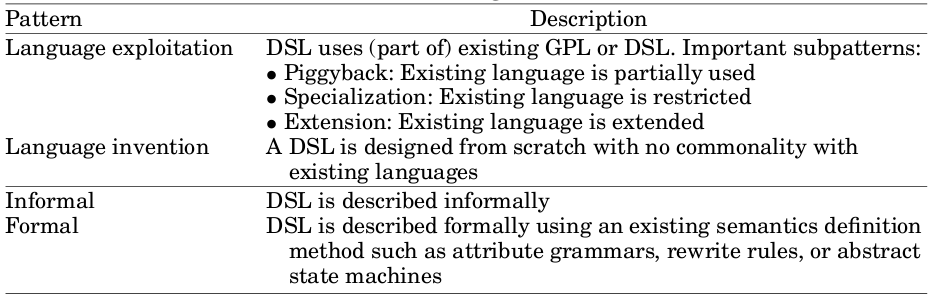
\includegraphics[width=\columnwidth]{img/designPatterns.png}
        \caption{Design patterns - Figure extracted of~\cite{mernik:2005}.}\label{fig:patterns}
\end{figure}

In the implementation is constructed a library with the semantic notations
together with a compiler that perfoms the lexical, syntactic and semantic analysis, 
after converts the DSL programs to sequence of library calls. Generally the library
and the compiler are constructed with support of the tools or framework developed
for this purpose. \textbf{Xtext}~\cite{xtext} and \textbf{Groovy}~\cite{groovyDSL, groovyDSLBook}
are good examples of tools to develop DSLs quickly.

\section{Context Transformation}

The bacteriological algorithm is part of the family of genetic algorithms that
works on genetic context. A minor particle this algorithm is a gene, but without
minor importance, all changes are influenced by it. The genes when clustered form
an individual that have more representativeness than an gene and the top is the
population that is set of individuals.

Our context is focused on hadoop environment that have your particularities. Thus
a context transformation is mandatory to implement the bacterionlogical algorithm
on such environment. This is not a complicated task for who know the hadoop
environment that is our specific domain.

On hadoop there is huge set of configuration parameters, we called one specific 
parameters of \textbf{knob}, but a job use several knobs that are one knobs set. 
When some knobs set are gathered we have a population of knobs.

So pure and simples tranformation have been done where each component of genetic
context were translated to one component of hadoop environment. Like shown in the
figure~\ref{fig:transformation} we can realize that one gene was transformed to one knob,
one individual(that is a genes set) was transformed to one knobs set and one individuals
population was transformed to knobs population.

\begin{figure}[htbp]
        \centering
        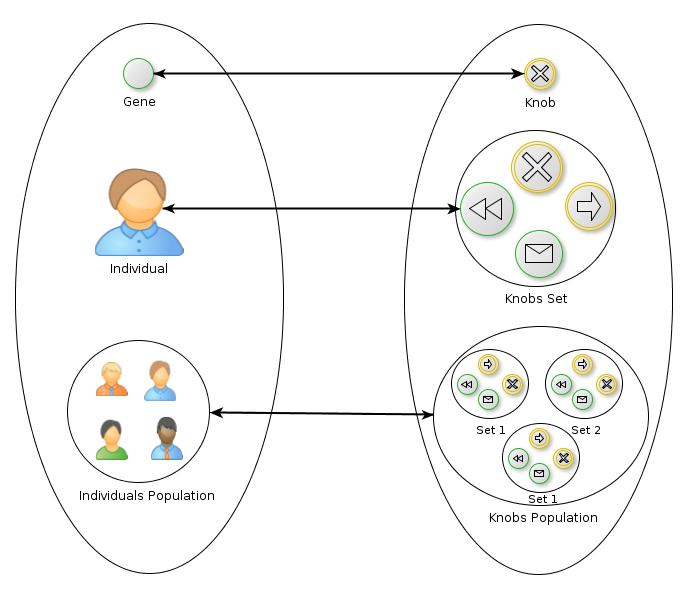
\includegraphics[width=\columnwidth]{img/transformation.jpg}
        \caption{Context transformation.}\label{fig:transformation}
\end{figure}

An interesting characteristic of the tranformation is its bijection that one
component in genetic domain is translated to one component in hadoop domain. Beyond
that the transformation has inversion property, i.e, all components in hadoop domain
can be translated to respective components in genetic domain. That properties
represent compatibility between both domains and somewhat a good representativeness.

\section{DSL Proposal}

The base of our DSL proposal is context transformation already explained, but to
develop the DLS still missing one library or framework that help us in this task.
The \textbf{Xtext}~\cite{xtext} framework seems one good option because is simple,
covers all our necessities and we already have knowledge with this tool.

Our effort concentrate in one MapRedue job and your knobs to be adjusted. One
draft of DLS is shown above:

\singlespacing
\begin{listing}[H]
\begin{minted}[mathescape,frame=lines,framesep=2mm,fontfamily=courier,fontsize=\scriptsize]{python}
DomainModel:
	job=Job;
	
Job:
	'Job' name=ID '{'
		setKnobs+=Knobs*
	'}'
;
	
Knobs:
	'knobs' '{'
		knobs+=Knob*
	'}' 
;

Knob:
	 name=ID Type
;

Type:
	IntType | FloatType | BoolType
;

IntType:
	'int' MinInt MaxInt '=' INT
;
MaxInt: INT;
MinInt: INT;

FloatType:
	'float' MinFloat MaxFloat '=' Float
;
MaxFloat: Float;
MinFloat: Float;

Float:
	INT*'.'INT*
;

BoolType:
	'boolean' '=' Boolean
;
Boolean:
	'true' | 'false' 
;

\end{minted}
\caption{Initial DSL proposal} 
\label{listing:dlsProposal}
\end{listing}

Let's explain all rules involving our grammar:
\begin{enumerate}
	\item
		\singlespacing
		\begin{listing}[H]
		\begin{minted}[mathescape,frame=lines,framesep=2mm,fontfamily=courier,fontsize=\scriptsize]{python}
			DomainModel:
				job=Job;
		\end{minted}
		\label{listing:modelRule}
		\end{listing}

		The first rule in a grammar is always used as the entry or start rule.
		It says that the \textbf{DomainModel} contains one element \textbf{Job}
		assigned to a feature called \textit{job}.

	\item
		\singlespacing
		\begin{listing}[H]
		\begin{minted}[mathescape,frame=lines,framesep=2mm,fontfamily=courier,fontsize=\scriptsize]{python}
			Job:
				'Job' name=ID '{'
					setKnobs+=Knobs*
				'}'
			;	
		\end{minted}
		\label{listing:modelRule}
		\end{listing}

		The rule \textbf{Job} starts with the definition of a keyword ({\it Job})
		followed by a name. Between 'braces' the job contains one arbitrary number
		(*) of \textbf{Knobs} which will be added (+=) to a feature called setKnobs.

	\item
		\singlespacing
		\begin{listing}[H]
		\begin{minted}[mathescape,frame=lines,framesep=2mm,fontfamily=courier,fontsize=\scriptsize]{python}
			Knobs:
				'knobs' '{'
					knobs+=Knob*
				'}' 
			;
		\end{minted}
		\label{listing:modelRule}
		\end{listing}

		The rule \textbf{Knobs} starts with the definition of a keyword {\bf knobs}
		and between 'braces' contains one arbitrary number (*) of \textbf{Knob}
		which will be added (+=) to a feature called knobs.

	\item
		\singlespacing
		\begin{listing}[H]
		\begin{minted}[mathescape,frame=lines,framesep=2mm,fontfamily=courier,fontsize=\scriptsize]{python}
			Knob:
				 name=ID Type
			;
		\end{minted}
		\label{listing:modelRule}
		\end{listing}

		The rule \textbf{Knob} contain one name followed by a \textbf{Type} with
		your peculiarities explained below.

	\item
		\singlespacing
		\begin{listing}[H]
		\begin{minted}[mathescape,frame=lines,framesep=2mm,fontfamily=courier,fontsize=\scriptsize]{python}
			Type:
				IntType | FloatType | BoolType
			;
		\end{minted}
		\label{listing:modelRule}
		\end{listing}

		The rule \textbf{Type} can accept three type: integer, float or boolean,
		this three are all possibles types on hadoop parameters configuration.

	\item
		\singlespacing
		\begin{listing}[H]
		\begin{minted}[mathescape,frame=lines,framesep=2mm,fontfamily=courier,fontsize=\scriptsize]{python}
			IntType:
				'int' MinInt MaxInt '=' INT
			;
			MaxInt: INT;
			MinInt: INT;
		\end{minted}
		\label{listing:modelRule}
		\end{listing}

		This three rules are used for integer types, the rule \textbf{IntType}
		starts with the keyword {\bf int} followed by your respective minimum
		and maximum possibles values. In sequence there is the keyword {\bf =}
		and the initial value for the knob.

	\item
		\singlespacing
		\begin{listing}[H]
		\begin{minted}[mathescape,frame=lines,framesep=2mm,fontfamily=courier,fontsize=\scriptsize]{python}
			FloatType:
				'float' MinFloat MaxFloat '=' Float
			;
			MaxFloat: Float;
			MinFloat: Float;

			Float:
				INT*'.'INT*
			;
		\end{minted}
		\label{listing:modelRule}
		\end{listing}

		This four rules are used for float types, the rule \textbf{FloatType} is
		similar the IntType rule, it starts with the keyword {\bf float} followed
		by your respective minimum and maximum possibles values. In sequence there
		is the key word {\bf =}	and the initial float value for the knob. The rule
		{\bf FloatType} expresses the float format.

	\item
		\singlespacing
		\begin{listing}[H]
		\begin{minted}[mathescape,frame=lines,framesep=2mm,fontfamily=courier,fontsize=\scriptsize]{python}
			BoolType:
				'boolean' '=' Boolean
			;
			Boolean:
				'true' | 'false' 
			;
		\end{minted}
		\label{listing:modelRule}
		\end{listing}

		The last one rule {\bf BoolType} expresses the boolean type, it starts with
		the keyword {\bf boolean} followed by signal of \textbf{=} and the initial
		boolean	value that can be {\bf true} or {\bf false}.

\end{enumerate}
